% Options for packages loaded elsewhere
\PassOptionsToPackage{unicode}{hyperref}
\PassOptionsToPackage{hyphens}{url}
%
\documentclass[
]{article}
\usepackage{lmodern}
\usepackage{amssymb,amsmath}
\usepackage{ifxetex,ifluatex}
\ifnum 0\ifxetex 1\fi\ifluatex 1\fi=0 % if pdftex
  \usepackage[T1]{fontenc}
  \usepackage[utf8]{inputenc}
  \usepackage{textcomp} % provide euro and other symbols
\else % if luatex or xetex
  \usepackage{unicode-math}
  \defaultfontfeatures{Scale=MatchLowercase}
  \defaultfontfeatures[\rmfamily]{Ligatures=TeX,Scale=1}
\fi
% Use upquote if available, for straight quotes in verbatim environments
\IfFileExists{upquote.sty}{\usepackage{upquote}}{}
\IfFileExists{microtype.sty}{% use microtype if available
  \usepackage[]{microtype}
  \UseMicrotypeSet[protrusion]{basicmath} % disable protrusion for tt fonts
}{}
\makeatletter
\@ifundefined{KOMAClassName}{% if non-KOMA class
  \IfFileExists{parskip.sty}{%
    \usepackage{parskip}
  }{% else
    \setlength{\parindent}{0pt}
    \setlength{\parskip}{6pt plus 2pt minus 1pt}}
}{% if KOMA class
  \KOMAoptions{parskip=half}}
\makeatother
\usepackage{xcolor}
\IfFileExists{xurl.sty}{\usepackage{xurl}}{} % add URL line breaks if available
\IfFileExists{bookmark.sty}{\usepackage{bookmark}}{\usepackage{hyperref}}
\hypersetup{
  pdftitle={Assignment 4: K Means Clustering},
  hidelinks,
  pdfcreator={LaTeX via pandoc}}
\urlstyle{same} % disable monospaced font for URLs
\usepackage[margin=1in]{geometry}
\usepackage{color}
\usepackage{fancyvrb}
\newcommand{\VerbBar}{|}
\newcommand{\VERB}{\Verb[commandchars=\\\{\}]}
\DefineVerbatimEnvironment{Highlighting}{Verbatim}{commandchars=\\\{\}}
% Add ',fontsize=\small' for more characters per line
\usepackage{framed}
\definecolor{shadecolor}{RGB}{248,248,248}
\newenvironment{Shaded}{\begin{snugshade}}{\end{snugshade}}
\newcommand{\AlertTok}[1]{\textcolor[rgb]{0.94,0.16,0.16}{#1}}
\newcommand{\AnnotationTok}[1]{\textcolor[rgb]{0.56,0.35,0.01}{\textbf{\textit{#1}}}}
\newcommand{\AttributeTok}[1]{\textcolor[rgb]{0.77,0.63,0.00}{#1}}
\newcommand{\BaseNTok}[1]{\textcolor[rgb]{0.00,0.00,0.81}{#1}}
\newcommand{\BuiltInTok}[1]{#1}
\newcommand{\CharTok}[1]{\textcolor[rgb]{0.31,0.60,0.02}{#1}}
\newcommand{\CommentTok}[1]{\textcolor[rgb]{0.56,0.35,0.01}{\textit{#1}}}
\newcommand{\CommentVarTok}[1]{\textcolor[rgb]{0.56,0.35,0.01}{\textbf{\textit{#1}}}}
\newcommand{\ConstantTok}[1]{\textcolor[rgb]{0.00,0.00,0.00}{#1}}
\newcommand{\ControlFlowTok}[1]{\textcolor[rgb]{0.13,0.29,0.53}{\textbf{#1}}}
\newcommand{\DataTypeTok}[1]{\textcolor[rgb]{0.13,0.29,0.53}{#1}}
\newcommand{\DecValTok}[1]{\textcolor[rgb]{0.00,0.00,0.81}{#1}}
\newcommand{\DocumentationTok}[1]{\textcolor[rgb]{0.56,0.35,0.01}{\textbf{\textit{#1}}}}
\newcommand{\ErrorTok}[1]{\textcolor[rgb]{0.64,0.00,0.00}{\textbf{#1}}}
\newcommand{\ExtensionTok}[1]{#1}
\newcommand{\FloatTok}[1]{\textcolor[rgb]{0.00,0.00,0.81}{#1}}
\newcommand{\FunctionTok}[1]{\textcolor[rgb]{0.00,0.00,0.00}{#1}}
\newcommand{\ImportTok}[1]{#1}
\newcommand{\InformationTok}[1]{\textcolor[rgb]{0.56,0.35,0.01}{\textbf{\textit{#1}}}}
\newcommand{\KeywordTok}[1]{\textcolor[rgb]{0.13,0.29,0.53}{\textbf{#1}}}
\newcommand{\NormalTok}[1]{#1}
\newcommand{\OperatorTok}[1]{\textcolor[rgb]{0.81,0.36,0.00}{\textbf{#1}}}
\newcommand{\OtherTok}[1]{\textcolor[rgb]{0.56,0.35,0.01}{#1}}
\newcommand{\PreprocessorTok}[1]{\textcolor[rgb]{0.56,0.35,0.01}{\textit{#1}}}
\newcommand{\RegionMarkerTok}[1]{#1}
\newcommand{\SpecialCharTok}[1]{\textcolor[rgb]{0.00,0.00,0.00}{#1}}
\newcommand{\SpecialStringTok}[1]{\textcolor[rgb]{0.31,0.60,0.02}{#1}}
\newcommand{\StringTok}[1]{\textcolor[rgb]{0.31,0.60,0.02}{#1}}
\newcommand{\VariableTok}[1]{\textcolor[rgb]{0.00,0.00,0.00}{#1}}
\newcommand{\VerbatimStringTok}[1]{\textcolor[rgb]{0.31,0.60,0.02}{#1}}
\newcommand{\WarningTok}[1]{\textcolor[rgb]{0.56,0.35,0.01}{\textbf{\textit{#1}}}}
\usepackage{graphicx,grffile}
\makeatletter
\def\maxwidth{\ifdim\Gin@nat@width>\linewidth\linewidth\else\Gin@nat@width\fi}
\def\maxheight{\ifdim\Gin@nat@height>\textheight\textheight\else\Gin@nat@height\fi}
\makeatother
% Scale images if necessary, so that they will not overflow the page
% margins by default, and it is still possible to overwrite the defaults
% using explicit options in \includegraphics[width, height, ...]{}
\setkeys{Gin}{width=\maxwidth,height=\maxheight,keepaspectratio}
% Set default figure placement to htbp
\makeatletter
\def\fps@figure{htbp}
\makeatother
\setlength{\emergencystretch}{3em} % prevent overfull lines
\providecommand{\tightlist}{%
  \setlength{\itemsep}{0pt}\setlength{\parskip}{0pt}}
\setcounter{secnumdepth}{-\maxdimen} % remove section numbering

\title{Assignment 4: K Means Clustering}
\author{}
\date{\vspace{-2.5em}}

\begin{document}
\maketitle

In this assignment we will be applying the K-means clustering algorithm
we looked at in class. At the following link you can find a description
of K-means:

\url{https://www.cs.uic.edu/~wilkinson/Applets/cluster.html}

\begin{Shaded}
\begin{Highlighting}[]
\KeywordTok{library}\NormalTok{(tidyverse)}
\end{Highlighting}
\end{Shaded}

\begin{verbatim}
## -- Attaching packages --------------------------------------- tidyverse 1.3.0 --
\end{verbatim}

\begin{verbatim}
## v ggplot2 3.3.2     v purrr   0.3.4
## v tibble  3.0.4     v dplyr   1.0.2
## v tidyr   1.1.2     v stringr 1.4.0
## v readr   1.4.0     v forcats 0.5.0
\end{verbatim}

\begin{verbatim}
## Warning: package 'tibble' was built under R version 4.0.3
\end{verbatim}

\begin{verbatim}
## -- Conflicts ------------------------------------------ tidyverse_conflicts() --
## x dplyr::filter() masks stats::filter()
## x dplyr::lag()    masks stats::lag()
\end{verbatim}

\begin{Shaded}
\begin{Highlighting}[]
\KeywordTok{library}\NormalTok{(STAT)}
\end{Highlighting}
\end{Shaded}

\begin{verbatim}
## Warning: package 'STAT' was built under R version 4.0.3
\end{verbatim}

Now, upload the file ``Class\_Motivation.csv'' from the Assignment 4
Repository as a data frame called ``K1''"

\begin{Shaded}
\begin{Highlighting}[]
\NormalTok{K1 <-}\StringTok{ }\KeywordTok{read.csv}\NormalTok{(}\StringTok{"Class_Motivation.csv"}\NormalTok{)}
\end{Highlighting}
\end{Shaded}

This file contains the self-reported motivation scores for a class over
five weeks. We are going to look for patterns in motivation over this
time and sort people into clusters based on those patterns.

But before we do that, we will need to manipulate the data frame into a
structure that can be analyzed by our clustering algorithm.

The algorithm will treat each row as a value belonging to a person, so
we need to remove the id variable.

\begin{Shaded}
\begin{Highlighting}[]
\NormalTok{K2 <-K1 }\OperatorTok\StringTok{  }\KeywordTok{select}\NormalTok{(}\OperatorTok{-}\NormalTok{id)}
\end{Highlighting}
\end{Shaded}

It is important to think about the meaning of missing values when
clustering. We could treat them as having meaning or we could remove
those people who have them. Neither option is ideal. What problems do
you foresee if we recode or remove these values? Write your answers
below:

We will remove people with missing values for this assignment, but keep
in mind the issues that you have identified.

\begin{Shaded}
\begin{Highlighting}[]
\NormalTok{K3 <-}\StringTok{ }\KeywordTok{na.omit}\NormalTok{(K2) }\CommentTok{#This command create a data frame with only those people with no missing values. It "omits" all rows with missing values, also known as a "listwise deletion". EG - It runs down the list deleting rows as it goes.}
\end{Highlighting}
\end{Shaded}

Another pre-processing step used in K-means is to standardize the values
so that they have the same range. We do this because we want to treat
each week as equally important - if we do not standardise then the week
with the largest range will have the greatest impact on which clusters
are formed. We standardise the values by using the ``scale()'' command.

\begin{Shaded}
\begin{Highlighting}[]
\NormalTok{K3 <-}\StringTok{ }\KeywordTok{scale}\NormalTok{(K3, }\DataTypeTok{center =} \OtherTok{TRUE}\NormalTok{, }\DataTypeTok{scale =} \OtherTok{TRUE}\NormalTok{)}
\end{Highlighting}
\end{Shaded}

Now we will run the K-means clustering algorithm we talked about in
class. 1) The algorithm starts by randomly choosing some starting values
2) Associates all observations near to those values with them 3)
Calculates the mean of those clusters of values 4) Selects the
observation closest to the mean of the cluster 5) Re-associates all
observations closest to this observation 6) Continues this process until
the clusters are no longer changing

Notice that in this case we have 5 variables and in class we only had 2.
It is impossible to vizualise this process with 5 variables.

Also, we need to choose the number of clusters we think are in the data.
We will start with 2.

\begin{Shaded}
\begin{Highlighting}[]
\NormalTok{fit <-}\StringTok{ }\KeywordTok{kmeans}\NormalTok{(K3,}\DecValTok{2}\NormalTok{)}

\CommentTok{#We have created an object called "fit" that contains all the details of our clustering including which observations belong to each cluster.}

\CommentTok{#We can access the list of clusters by typing "fit$cluster", the top row corresponds to the original order the rows were in. Notice we have deleted some rows.}



\CommentTok{#We can also attach these clusters to the original dataframe by using the "data.frame" command to create a new data frame called K4.}

\NormalTok{K4 <-}\StringTok{ }\KeywordTok{data.frame}\NormalTok{(K3,fit}\OperatorTok{$}\NormalTok{cluster)}

\CommentTok{#Have a look at the K4 dataframe. Lets change the names of the variables to make it more convenient with the names() command.}
\KeywordTok{names}\NormalTok{(K4) <-}\StringTok{ }\KeywordTok{c}\NormalTok{(}\StringTok{"1"}\NormalTok{,}\StringTok{"2"}\NormalTok{,}\StringTok{"3"}\NormalTok{,}\StringTok{"4"}\NormalTok{,}\StringTok{"5"}\NormalTok{,}\StringTok{"cluster"}\NormalTok{)}
\end{Highlighting}
\end{Shaded}

Now we need to visualize the clusters we have created. To do so we want
to play with the structure of our data. What would be most useful would
be if we could visualize average motivation by cluster, by week. To do
this we will need to convert our data from wide to long format. Remember
your old friends tidyr and dplyr!

First lets use tidyr to convert from wide to long format.

\begin{Shaded}
\begin{Highlighting}[]
\NormalTok{K5 <-}\StringTok{ }\KeywordTok{gather}\NormalTok{(K4, }\StringTok{"week"}\NormalTok{, }\StringTok{"motivation"}\NormalTok{, }\DecValTok{1}\OperatorTok{:}\DecValTok{5}\NormalTok{)}
\end{Highlighting}
\end{Shaded}

Now lets use dplyr to average our motivation values by week and by
cluster.

\begin{Shaded}
\begin{Highlighting}[]
\NormalTok{K6 <-}\StringTok{ }\NormalTok{K5 }\OperatorTok\StringTok{ }\KeywordTok{group_by}\NormalTok{(week, cluster) }\OperatorTok\StringTok{ }\KeywordTok{summarise}\NormalTok{(}\DataTypeTok{avg =} \KeywordTok{mean}\NormalTok{(motivation))}
\end{Highlighting}
\end{Shaded}

\begin{verbatim}
## `summarise()` regrouping output by 'week' (override with `.groups` argument)
\end{verbatim}

Now it's time to do some visualization:

\url{https://www.cs.uic.edu/~wilkinson/TheGrammarOfGraphics/GOG.html}

And you can see the range of available graphics in ggplot here:

\url{http://ggplot2.tidyverse.org/reference/index.html}

We are going to create a line plot similar to the one created in this
paper about school dropout
\href{http://pareonline.net/pdf/v15n7.pdf}{Bowers, 2010}. It will have
motivation on the Y-axis and weeks on the X-axis. To do this we will
want our weeks variables to be treated as a number, but because it was
created from a variable name it is currently being treated as a
character variable. You can see this if you click on the arrow on the
left of K6 in the Data pane. Week is designated by ``chr''. To convert
it to numeric, we use the as.numeric command.

Likewise, since ``cluster'' is not numeric but rather a categorical
label we want to convert it from an ``integer'' format to a ``factor''
format so that ggplot does not treat it as a number. We can do this with
the as.factor() command.

\begin{Shaded}
\begin{Highlighting}[]
\NormalTok{K6}\OperatorTok{$}\NormalTok{week <-}\StringTok{ }\KeywordTok{as.numeric}\NormalTok{(K6}\OperatorTok{$}\NormalTok{week)}

\NormalTok{K6}\OperatorTok{$}\NormalTok{cluster <-}\StringTok{ }\KeywordTok{as.factor}\NormalTok{(K6}\OperatorTok{$}\NormalTok{cluster)}
\end{Highlighting}
\end{Shaded}

Now we can plot our line plot using the ggplot command, ``ggplot()''.

\begin{itemize}
\tightlist
\item
  The first argument in a ggplot is the dataframe we are using: K6
\item
  Next is what is called an aesthetic (aes), the aesthetic tells ggplot
  which variables to use and how to use them. Here we are using the
  variables ``week'' and ``avg'' on the x and y axes and we are going
  color these variables using the ``cluster'' variable
\item
  Then we are going to tell ggplot which type of plot we want to use by
  specifiying a ``geom()'', in this case a line plot: geom\_line()
\item
  Finally we are going to clean up our axes labels: xlab(``Week'') \&
  ylab(``Average Motivation'')
\end{itemize}

\begin{Shaded}
\begin{Highlighting}[]
\KeywordTok{ggplot}\NormalTok{(K6, }\KeywordTok{aes}\NormalTok{(week, avg, }\DataTypeTok{colour =}\NormalTok{ cluster)) }\OperatorTok{+}\StringTok{ }\KeywordTok{geom_line}\NormalTok{() }\OperatorTok{+}\StringTok{ }\KeywordTok{xlab}\NormalTok{(}\StringTok{"Week"}\NormalTok{) }\OperatorTok{+}\StringTok{ }\KeywordTok{ylab}\NormalTok{(}\StringTok{"Average Motivation"}\NormalTok{)}
\end{Highlighting}
\end{Shaded}

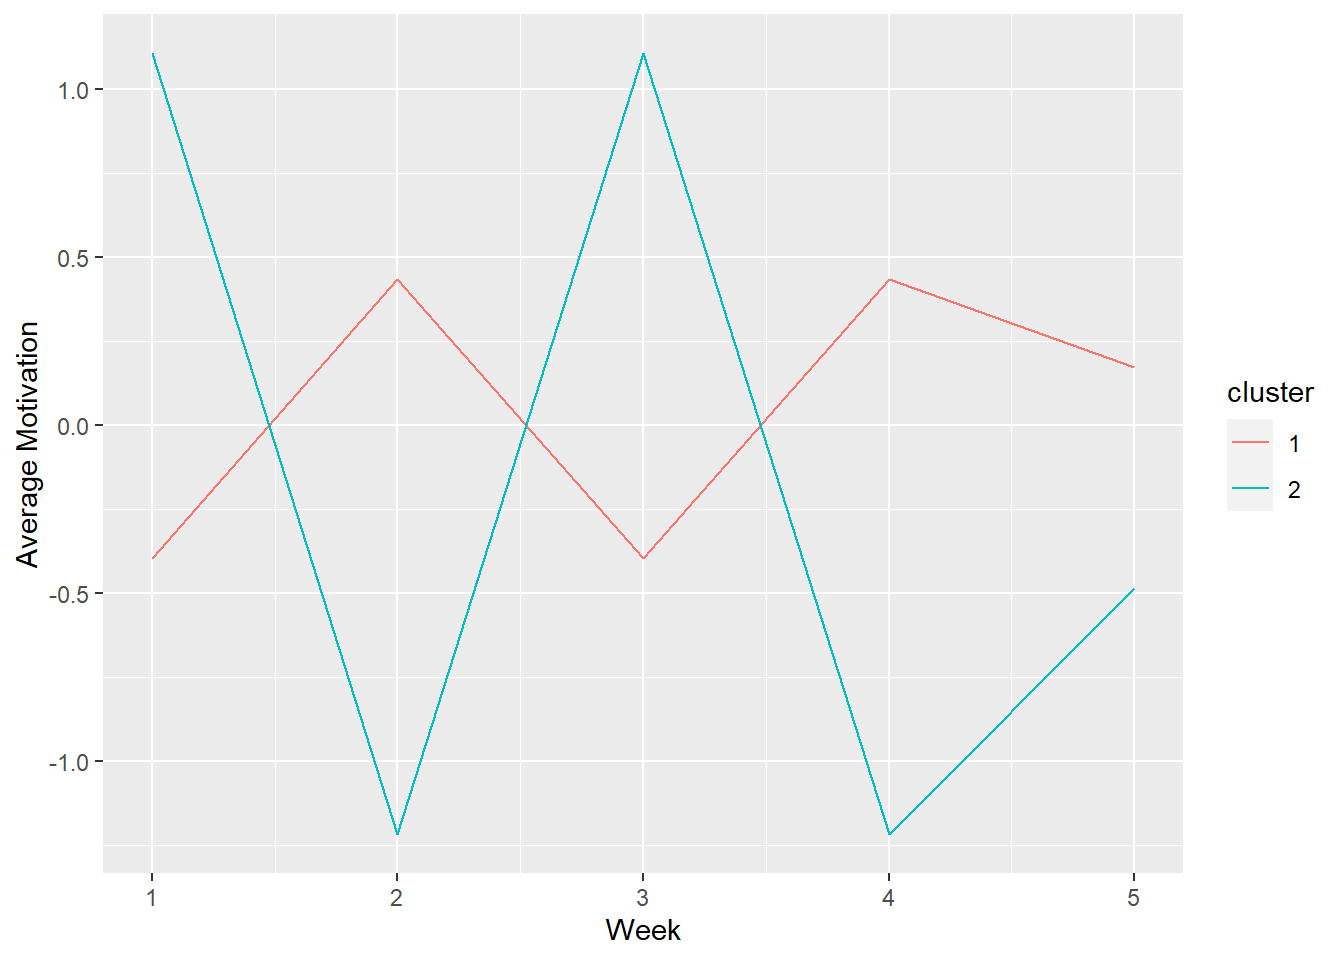
\includegraphics{Assignment-4_files/figure-latex/unnamed-chunk-10-1.pdf}

What patterns do you see in the plot?

As the motivation of cluster 1 increased, the motivation of cluster 2
decreased and vice-versa. The Cluster were mirror opposite of each
other.

It would be useful to determine how many people are in each cluster. We
can do this easily with dplyr.

\begin{Shaded}
\begin{Highlighting}[]
\NormalTok{K7 <-}\StringTok{ }\KeywordTok{count}\NormalTok{(K4, cluster)}
\end{Highlighting}
\end{Shaded}

Look at the number of people in each cluster, now repeat this process
for 3 rather than 2 clusters. Which cluster grouping do you think is
more informative? Write your answer below:

\#\#Part II

Using the data collected in the HUDK4050 entrance survey
(HUDK4050-cluster.csv) use K-means to cluster the students first
according location (lat/long) and then according to their answers to the
questions, each student should belong to two clusters.

Read the file and clear up

\begin{Shaded}
\begin{Highlighting}[]
\KeywordTok{library}\NormalTok{(janitor)}
\end{Highlighting}
\end{Shaded}

\begin{verbatim}
## Warning: package 'janitor' was built under R version 4.0.3
\end{verbatim}

\begin{verbatim}
## 
## Attaching package: 'janitor'
\end{verbatim}

\begin{verbatim}
## The following objects are masked from 'package:stats':
## 
##     chisq.test, fisher.test
\end{verbatim}

\begin{Shaded}
\begin{Highlighting}[]
\NormalTok{ES <-}\KeywordTok{read.csv}\NormalTok{(}\StringTok{"HUDK405020-cluster.csv"}\NormalTok{, }\DataTypeTok{header =} \OtherTok{TRUE}\NormalTok{)}
\CommentTok{#make a tibble, clean names, and remove empty rows and columns}
\NormalTok{ES1 <-}\StringTok{ }\KeywordTok{as_tibble}\NormalTok{(ES) }\OperatorTok\StringTok{ }\KeywordTok{clean_names}\NormalTok{() }\OperatorTok\StringTok{ }\KeywordTok{remove_empty}\NormalTok{()}
\end{Highlighting}
\end{Shaded}

\begin{verbatim}
## value for "which" not specified, defaulting to c("rows", "cols")
\end{verbatim}

\begin{Shaded}
\begin{Highlighting}[]
\CommentTok{#finding duplicates}
\NormalTok{Dupes <-}\StringTok{ }\NormalTok{ES1 }\OperatorTok\StringTok{ }\KeywordTok{get_dupes}\NormalTok{()}
\end{Highlighting}
\end{Shaded}

\begin{verbatim}
## No variable names specified - using all columns.
\end{verbatim}

\begin{verbatim}
## No duplicate combinations found of: id, lat, long, compare_features, math_accuracy, planner_use, enjoy_discuss, enjoy_group, meet_deadline
\end{verbatim}

\begin{Shaded}
\begin{Highlighting}[]
\CommentTok{#No duplicates}
\CommentTok{#Changing id to character so it is not treated as an integer}
\NormalTok{ES1}\OperatorTok{$}\NormalTok{id <-}\StringTok{ }\KeywordTok{as.character}\NormalTok{(ES1}\OperatorTok{$}\NormalTok{id)}
\end{Highlighting}
\end{Shaded}

Creating two tables. One for long/lat and one for questions

\begin{Shaded}
\begin{Highlighting}[]
\CommentTok{#location table}
\NormalTok{ESL <-}\StringTok{ }\NormalTok{ES1 }\OperatorTok\StringTok{ }\KeywordTok{select}\NormalTok{(}\DecValTok{2}\OperatorTok{:}\DecValTok{3}\NormalTok{) }
\CommentTok{#question table}
\NormalTok{ESQ <-}\StringTok{ }\NormalTok{ES1 }\OperatorTok\StringTok{ }\KeywordTok{select}\NormalTok{(}\DecValTok{4}\OperatorTok{:}\DecValTok{9}\NormalTok{)}
\end{Highlighting}
\end{Shaded}

\#\#K Means clustering - Location table Exploratory Clustering I am
going to use the broom package, and experiment with a method I found on
the Tidyverse page to create multiple models to decide the number of
clusters I should be using. In addition, I know from the week 2 video
(2.2) ``Visual Analysis of the Student Survey'' there is the possibility
of 3+ clusters (2 in the USA + China + others).

\begin{Shaded}
\begin{Highlighting}[]
\KeywordTok{library}\NormalTok{(broom)}
\end{Highlighting}
\end{Shaded}

\begin{verbatim}
## Warning: package 'broom' was built under R version 4.0.3
\end{verbatim}

\begin{Shaded}
\begin{Highlighting}[]
\CommentTok{#Nesting the K-means Clustering}
\NormalTok{kclust <-}\StringTok{ }
\StringTok{  }\KeywordTok{tibble}\NormalTok{(}\DataTypeTok{k =} \DecValTok{1}\OperatorTok{:}\DecValTok{5}\NormalTok{) }\OperatorTok\StringTok{ }
\StringTok{  }\KeywordTok{mutate}\NormalTok{(}
    \DataTypeTok{kclust =} \KeywordTok{map}\NormalTok{(k, }\OperatorTok{~}\KeywordTok{kmeans}\NormalTok{(ESL, .x)),}
    \DataTypeTok{tidied =} \KeywordTok{map}\NormalTok{(kclust, tidy),}
    \DataTypeTok{glanced =} \KeywordTok{map}\NormalTok{(kclust, glance),}
    \DataTypeTok{augmented =} \KeywordTok{map}\NormalTok{(kclust, augment, ESL)}
\NormalTok{  )}
\CommentTok{#creating 3 data sets to create exploratory visualization}
\NormalTok{centers <-}\StringTok{ }
\StringTok{  }\NormalTok{kclust }\OperatorTok
\StringTok{  }\KeywordTok{unnest}\NormalTok{(}\DataTypeTok{cols =} \KeywordTok{c}\NormalTok{(tidied))}

\NormalTok{clusters <-}\StringTok{ }
\StringTok{  }\NormalTok{kclust }\OperatorTok\StringTok{ }
\StringTok{  }\KeywordTok{unnest}\NormalTok{(}\DataTypeTok{cols =} \KeywordTok{c}\NormalTok{(augmented))}

\NormalTok{scree <-}\StringTok{ }
\StringTok{  }\NormalTok{kclust }\OperatorTok
\StringTok{  }\KeywordTok{unnest}\NormalTok{(}\DataTypeTok{cols =} \KeywordTok{c}\NormalTok{(glanced))}
\end{Highlighting}
\end{Shaded}

Exploratory visualization

\begin{Shaded}
\begin{Highlighting}[]
\CommentTok{#scatter plot}
\KeywordTok{ggplot}\NormalTok{(clusters, }\KeywordTok{aes}\NormalTok{(}\DataTypeTok{x =}\NormalTok{ lat, }\DataTypeTok{y =}\NormalTok{ long)) }\OperatorTok{+}
\StringTok{  }\KeywordTok{geom_point}\NormalTok{(}\KeywordTok{aes}\NormalTok{(}\DataTypeTok{color =}\NormalTok{ .cluster), }\DataTypeTok{alpha =} \FloatTok{.75}\NormalTok{) }\OperatorTok{+}\StringTok{ }
\StringTok{  }\KeywordTok{facet_wrap}\NormalTok{(}\OperatorTok{~}\StringTok{ }\NormalTok{k)}
\end{Highlighting}
\end{Shaded}

\includegraphics{Assignment-4_files/figure-latex/unnamed-chunk-15-1.pdf}

\begin{Shaded}
\begin{Highlighting}[]
\CommentTok{# based on my knowledge from the video it looks like I should be using 3 or 4 plots. I am going to make a scree plot just to experiment since that is the purpose of this class.}
\KeywordTok{ggplot}\NormalTok{(scree, }\KeywordTok{aes}\NormalTok{(k, tot.withinss)) }\OperatorTok{+}
\StringTok{  }\KeywordTok{geom_line}\NormalTok{() }\OperatorTok{+}
\StringTok{  }\KeywordTok{geom_point}\NormalTok{()}
\end{Highlighting}
\end{Shaded}

\includegraphics{Assignment-4_files/figure-latex/unnamed-chunk-15-2.pdf}

\begin{Shaded}
\begin{Highlighting}[]
\CommentTok{# it appears I should be using 2 clusters, but I am going to sue 4 based on my knowledge that there are two groups in the USA and a significant amount of students in China. THe scree plot helped me realized that 4 too any clusters.}
\end{Highlighting}
\end{Shaded}

Location K-mean clusters

\begin{Shaded}
\begin{Highlighting}[]
\NormalTok{Loc <-}\StringTok{ }\KeywordTok{kmeans}\NormalTok{(ESL, }\DataTypeTok{centers =} \DecValTok{3}\NormalTok{)}
\CommentTok{#augment to extract the cluster number info}
\NormalTok{LocClust <-}\StringTok{ }\KeywordTok{augment}\NormalTok{(Loc,ES1) }\OperatorTok\StringTok{ }\KeywordTok{select}\NormalTok{(}\OperatorTok{-}\DecValTok{4}\OperatorTok{:-}\DecValTok{9}\NormalTok{) }\OperatorTok\StringTok{ }\KeywordTok{rename}\NormalTok{(}\DataTypeTok{LocClust=}\NormalTok{.cluster)}
\end{Highlighting}
\end{Shaded}

\#\#K Means clustering - Questions I am running a scree plot to practice

\begin{Shaded}
\begin{Highlighting}[]
\NormalTok{KclustQ <-}\StringTok{ }
\StringTok{  }\KeywordTok{tibble}\NormalTok{(}\DataTypeTok{k =} \DecValTok{1}\OperatorTok{:}\DecValTok{5}\NormalTok{) }\OperatorTok\StringTok{ }
\StringTok{  }\KeywordTok{mutate}\NormalTok{(}
    \DataTypeTok{kclust =} \KeywordTok{map}\NormalTok{(k, }\OperatorTok{~}\KeywordTok{kmeans}\NormalTok{(ESQ, .x)),}
    \DataTypeTok{tidied =} \KeywordTok{map}\NormalTok{(kclust, tidy),}
    \DataTypeTok{glanced =} \KeywordTok{map}\NormalTok{(kclust, glance),}
    \DataTypeTok{augmented =} \KeywordTok{map}\NormalTok{(kclust, augment, ESL)}
\NormalTok{  )}
\CommentTok{#Extract the data}
\NormalTok{screeQ <-}\StringTok{ }
\StringTok{  }\NormalTok{KclustQ }\OperatorTok
\StringTok{  }\KeywordTok{unnest}\NormalTok{(}\DataTypeTok{cols =} \KeywordTok{c}\NormalTok{(glanced))}
\CommentTok{#Scree plot}
\KeywordTok{ggplot}\NormalTok{(screeQ , }\KeywordTok{aes}\NormalTok{(k, tot.withinss)) }\OperatorTok{+}
\StringTok{  }\KeywordTok{geom_line}\NormalTok{() }\OperatorTok{+}
\StringTok{  }\KeywordTok{geom_point}\NormalTok{()}
\end{Highlighting}
\end{Shaded}

\includegraphics{Assignment-4_files/figure-latex/unnamed-chunk-17-1.pdf}

\begin{Shaded}
\begin{Highlighting}[]
\CommentTok{#No clear drop off, but I am going to use 3 again as it appears the drop off is between 2-3,a nd people in education love to group people in 3-4 groups (e.g., low, medium, high).}

\CommentTok{# Now that I have experimented, I think it would be interesting to use the within and other info that is available rather than do it by exploratory visuals}
\end{Highlighting}
\end{Shaded}

Question Clusters

\begin{Shaded}
\begin{Highlighting}[]
\NormalTok{Ques <-}\StringTok{ }\KeywordTok{kmeans}\NormalTok{(ESQ, }\DataTypeTok{centers =} \DecValTok{3}\NormalTok{)}
\CommentTok{#augment to extract the cluster number info}
\NormalTok{QClust <-}\StringTok{ }\KeywordTok{augment}\NormalTok{(Ques,ES1) }\OperatorTok\StringTok{ }\KeywordTok{select}\NormalTok{(}\OperatorTok{-}\DecValTok{2}\OperatorTok{:-}\DecValTok{3}\NormalTok{) }\OperatorTok\StringTok{ }\KeywordTok{rename}\NormalTok{(}\DataTypeTok{Qclust=}\NormalTok{.cluster)}
\end{Highlighting}
\end{Shaded}

\#\#Part III

Create a visualization that shows the overlap between the two clusters
each student belongs to in Part II. IE - Are there geographical patterns
that correspond to the answers? It doesnt appear as if there is a
relatio

\begin{Shaded}
\begin{Highlighting}[]
\CommentTok{#combine the cluster tables}

\NormalTok{clusters <-}\StringTok{ }\NormalTok{LocClust }\OperatorTok\StringTok{ }\KeywordTok{full_join}\NormalTok{(QClust, }\DataTypeTok{by=}\StringTok{"id"}\NormalTok{)}
\NormalTok{clusters <-}\StringTok{ }\NormalTok{clusters }\OperatorTok\StringTok{ }\KeywordTok{select}\NormalTok{(}\DecValTok{1}\NormalTok{,}\DecValTok{4}\NormalTok{,}\DecValTok{11}\NormalTok{)}
\NormalTok{clusters <-}\StringTok{ }\NormalTok{clusters }\OperatorTok\StringTok{ }\KeywordTok{rename}\NormalTok{(}\DataTypeTok{Location_Clusters=}\NormalTok{LocClust,}\DataTypeTok{Question_Clusters=}\NormalTok{Qclust)}
\NormalTok{cluster_table <-}\StringTok{ }\NormalTok{clusters }\OperatorTok\StringTok{  }
\StringTok{  }\KeywordTok{tabyl}\NormalTok{(Location_Clusters,Question_Clusters) }\CommentTok{#%>% }
 \CommentTok{# adorn_percentages("row") %>% }
 \CommentTok{# adorn_pct_formatting(rounding = "half up", digits = 0) %>%}
  \CommentTok{#adorn_ns() %>%}
 \CommentTok{# adorn_title("top",row_name = "Location Clusters", col_name = "Survey Question Clusters") %>%}
 \CommentTok{# knitr::kable()}
          
\KeywordTok{library}\NormalTok{(ztable)}
\end{Highlighting}
\end{Shaded}

\begin{verbatim}
## Warning: package 'ztable' was built under R version 4.0.3
\end{verbatim}

\begin{verbatim}
## Welcome to package ztable ver 0.2.2
\end{verbatim}

\begin{Shaded}
\begin{Highlighting}[]
\KeywordTok{options}\NormalTok{(}\DataTypeTok{ztable.type=}\StringTok{"html"}\NormalTok{)}
\NormalTok{z=}\KeywordTok{ztable}\NormalTok{(cluster_table)}
\NormalTok{Heatmap <-}\StringTok{ }\NormalTok{z }\OperatorTok\StringTok{ }\KeywordTok{makeHeatmap}\NormalTok{() }\OperatorTok\StringTok{ }\KeywordTok{print}\NormalTok{(}\DataTypeTok{caption=}\StringTok{"Geographic Pattern by Student Survey"}\NormalTok{)}
\end{Highlighting}
\end{Shaded}

\begin{verbatim}
## <head><style>
##         table {
##               font-family: times ;
## color:  black ;
## text-align: right;}
##         th {
##               padding: 1px 1px 5px 5px;
##          }
##         td {
##              padding: 1px 1px 5px 5px; }
##       </style></head><table align="center" style="border-collapse: collapse; caption-side:top; font-size:11pt;"><caption style="text-align:center;">Geographic Pattern by Student Survey</caption><tr>
## <th style="border-left: 0px solid black;background-color: #FFFFFF;border-top: 2px solid gray;border-bottom: 1px solid gray;">&nbsp;</th>
## <th <th align="center" style="font-weight: normal;border-left: 0px solid black;border-bottom: 1px solid gray;border-top: 2px solid gray;">Location_Clusters</th>
## <th <th align="center" style="font-weight: normal;border-left: 0px solid black;border-bottom: 1px solid gray;border-top: 2px solid gray;">1</th>
## <th <th align="center" style="font-weight: normal;border-left: 0px solid black;border-bottom: 1px solid gray;border-top: 2px solid gray;">2</th>
## <th <th align="center" style="font-weight: normal;border-left: 0px solid black;border-right:0px solid black;border-bottom: 1px solid gray;border-top: 2px solid gray;">3</th>
## </tr>
## <tr>
## <td  style="border-left: 0px solid black; ">1</td>
## <td align="left" style="border-left: 0px solid black;">1</td>
## <td align="right" style="border-left: 0px solid black;background-color: #FEE0D2;">8.00</td>
## <td align="right" style="border-left: 0px solid black;background-color: #FEE0D2;">8.00</td>
## <td align="right" style="border-left: 0px solid black;border-right:0px solid black;background-color: #FB6A4A;color: #FFFFFF;">11.00</td>
## </tr>
## <tr>
## <td  style="border-left: 0px solid black; border-top: hidden;">2</td>
## <td align="left" style="border-left: 0px solid black;border-top: hidden;">2</td>
## <td align="right" style="border-left: 0px solid black;border-top: hidden;background-color: #FEE0D2;">8.00</td>
## <td align="right" style="border-left: 0px solid black;border-top: hidden;background-color: #FB6A4A;color: #FFFFFF;">11.00</td>
## <td align="right" style="border-left: 0px solid black;border-right:0px solid black;border-top: hidden;background-color: #67000D;color: #FFFFFF;">17.00</td>
## </tr>
## <tr>
## <td  style="border-left: 0px solid black; border-top: hidden;">3</td>
## <td align="left" style="border-left: 0px solid black;border-top: hidden;">3</td>
## <td align="right" style="border-left: 0px solid black;border-top: hidden;background-color: #FEE0D2;">8.00</td>
## <td align="right" style="border-left: 0px solid black;border-top: hidden;background-color: #FFF5F0;">6.00</td>
## <td align="right" style="border-left: 0px solid black;border-right:0px solid black;border-top: hidden;background-color: #FEE0D2;">7.00</td>
## </tr>
## <tr>
## <td colspan="5" align="left" style="font-size:9pt ;border-top: 1px solid black; border-bottom: hidden;"></td>
## </tr>
## </table>
\end{verbatim}

\hypertarget{please-render-your-code-as-an-.html-file-using-knitr-and-pull-resquest-both-your-.rmd-file-and-.html-files-to-the-assignment-3-repository.}{%
\subsection{Please render your code as an .html file using knitr and
Pull Resquest both your .Rmd file and .html files to the Assignment 3
repository.}\label{please-render-your-code-as-an-.html-file-using-knitr-and-pull-resquest-both-your-.rmd-file-and-.html-files-to-the-assignment-3-repository.}}

\end{document}
